\documentclass[11pt,letterpaper]{article}
\usepackage{amsmath}
\usepackage{amsfonts}
\usepackage{amssymb}
\usepackage{fullpage}
\usepackage{graphicx}
\usepackage[normalem]{ulem}
\usepackage{url}
\usepackage{graphicx}

%1 Exercise number
%2 Exercise name
%3 Date performed
%4 Date submitted
\newcommand{\coversheet}[4]{
  \begin{titlepage}
    \setlength\topmargin{2in}
    \begin{center}
      \Huge\textsc{Smart Refrigerator Proposal}\\
      \vspace{.125in}
      \hrule
      \vspace{.125in}
      \normalsize
      \today \\
      \vspace{.375in}
      This project will develop a prototype “Smart Refrigerator” system, which will monitor grocery items purchased by the user in order to reduce food waste and facilitate efficient shopping habits. 

    \end{center}
    \vfill
    \hspace{4.2in} Steven Strapp - ses6498@rit.edu
    
    \noindent \hspace{4.2in} Computer Engineering Year 4

    \noindent \hspace{4.2in} 

    \noindent \hspace{4.2in} Ben Reeves - bpr5171@rit.edu
    
    \noindent \hspace{4.2in} Computer Engineering Year 5

    \noindent \hspace{4.2in} 

    \noindent \hspace{4.2in} Dustin Stroup - dxs2857@rit.edu

    \noindent \hspace{4.2in} Computer Engineering Year 5

    \quad \newline \newline \newline \newline \newline \newline \newline \newline
  \end{titlepage}
}

%1 label
%2 number of variables
%3 kmap label
%4 variables
%5 truth table
%6 Marks
%7 Prime implicants table
%8 Final EQ
\newcommand{\kmap}[8]{
  \begin{center}
    \begin{tabular}{l}
      \multicolumn{2}{c}{\underline{#1}} \\  
        \karnaughmap{#2}{#3}{#4}{#5}{
		#6        
        }
      #8
    \end{tabular}
  \end{center}
  }

%1 figure position
%2 figure scale
%3 path to photo
%4 Caption
%5 reference lable
\newcommand{\pic}[5]{
\begin{figure}[#1]
  \begin{center}
    \includegraphics[scale=#2]{#3}
    \caption{#4}
    \label{#5}
  \end{center}
\end{figure}
}


\begin{document}
\coversheet{V}{\textsc{Kinetis K60 Based Electrocardiogram}}{October 28, 2011}{November 11, 2011}
\setcounter{page}{2}

\tableofcontents
\pagebreak
\section{Overview}
\subsection{Needs Statement}
The New York Times reports that an average American family of four will account for over 120 pounds of food waste per month and that 27\% percent of all food available will be lost to waste \cite{times}. In addition, other resources are lost due to inefficient shopping practices; forgetting common items or special trips made for recipe ingredients waste time and fuel. A system is required for shoppers both to ensure their purchases are used before expiration and to assist in planning of grocery shopping trips.
\subsection{Objective Statement}
The objective of this project is to design a prototype that will allow a user to track food items in order to reduce waste and improve shopping efficiency. The system will remind the user about items nearing their expiration date and track the frequency of purchased items. From this frequency calculation the system will suggest typical shopping lists. A mobile phone application will provide an interface to the unit to view or create shopping lists and to query inventory.
\subsection{Brief Description}
A UPC scanner will be used to identify items added or removed from the refrigerator's inventory; a database of UPC codes will translate from the scanned code to an item description. Two databases will be maintained, one linking UPC codes to product descriptions and expiration dates and another to store items currently checked into the refrigerator. A central processing platform on the base station will be used to decode UPC information and to store and interact with the databases. This platform will provide a web interface accessible both via a large convenient display on the main unit and also using a mobile interface. The display on the main unit will allow a user both to check current inventory with expiration dates and to provide additional information when adding or removing items. Both the base station and mobile interfaces can also be used to display and modify suggested shopping lists. The mobile application will interact with the same web interface but will provide a graphical interface optimized for smaller displays. The system will continually estimate the frequency that particular items are purchased and will use this information combined with the expiration dates and purchase dates to suggest shopping lists.
\newline \quad \newline
A high level system diagram isolating components is shown below in Figure \ref{fig:sysdiag}.
\begin{figure}[h!]
\begin{center}
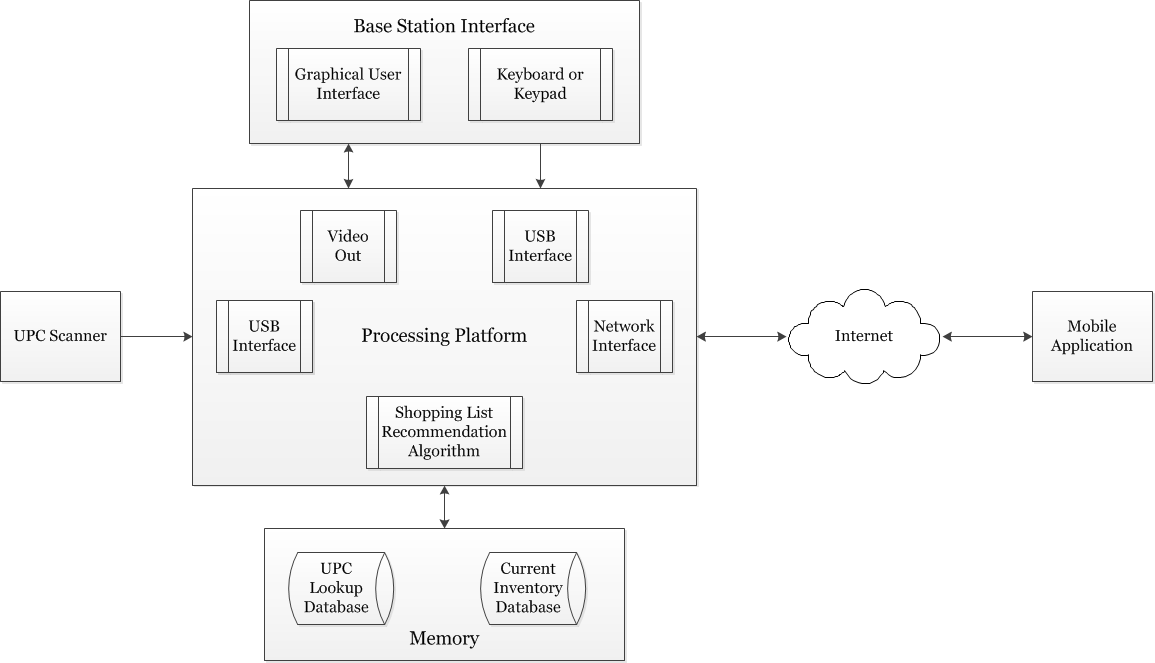
\includegraphics[scale=0.5]{SmartFridgeTopLevel}
\end{center}
\caption{High Level System Diagram}
\label{fig:sysdiag}
\end{figure}
\pagebreak
\section{Requirements Specification}
\subsection{Customer Needs}
\begin{enumerate}
\item The system should provide an intuitive, easy to use graphical interface.
\item The system should require minimal user input.
\item The system should be able to scan product codes and identify corresponding items quickly.
\item The system should provide secure remote access.
\item The system should report items nearing expiration.
\item The system should provide access to the current inventory.
\item The system should provide a method to create and edit shopping lists.
\item The system should recommend shopping lists which accurately reflect buying habits.
\item The system should function as an add-on to an existing refrigerator or pantry.
\end{enumerate}
\pagebreak
\subsection{Engineering Specifications}
\begin{table}[h!]
\begin{center}
\begin{tabular}{| p{1.2in} | p{2.5in} |p{2.5in} |}
\hline
Customer Need & Engineering Requirement & Justification \\
\hline
2,3 &A. An off-the-shelf UPC scanner should be used to input items. & A UPC scanner can read product codes with a single click.\\
\hline
3 &B. An internal UPC code database should be used to associate codes with items.&An internal database will remove delays associated with an internet look-up.\\
\hline
1,4,6&C. The system should be internet enabled and provide a web interface.&By providing a web interface any other internet-connected device can access the system.\\
\hline
4&D. Remote access should be authenticated with user name and password.&User names and passwords are standard for access control.\\
\hline
2,5&E. An internal database will store default recommended expiration estimates for common categories of items.&Inferring expiration dates based on item category helps minimizes user input. It is well known how long some products take to expire.\\
\hline
1,5&F. The user interface will provide a method for updating default expiration estimates.&Default estimates will not account for condition of product on arrival and may need to be updated.\\
\hline
1,5&G. Interface will provide a visual indication to the user when items are within a user-defined margin of expiration.&The goal of the system is to reduce waste due to expiration.\\
\hline
1,6&H. From both the base station and mobile application the user will be able to view an inventory list.&The user needs access to the current inventory in order to use items and shop effectively.\\
\hline
7,8&I. A database will be devoted to storing recommend shopping lists produced by the system.&User may wish to retain generic shopping lists for future use.\\
\hline
8&J. Recommended shopping lists will reflect purchasing history and expiration dates of current inventory.&Recommendation policy must suggest items relevant to the user in order to be useful.\\
\hline
7&K. Custom shopping lists, created either from the base station or the mobile interface, can be added to shopping list database.&Inefficient shopping practices can be prevented by storing shopping lists and the system can not anticipate all required items.\\
\hline
9&L. The system will be self-contained and no modifications will be required to existing appliances.&Similar systems are commercially available but require costly replacement of existing appliances.\\
\hline
\end{tabular}
\end{center}
\end{table}
\section{Concept Selection}
\subsection{Evaluation of Existing Systems}
Many refrigerator systems are current available which offer integrated displays and internet connectivity. LG, Electrolux, and Samsung all offer refrigerators with large LCD displays that provide access to calendar applications, recipes, weather forecasts, and music and photo sharing services. The principle shortcoming of these devices is the elevated price and the need to completely replace existing appliances. As a more affordable alternative, tablet mounts are available for refrigerators as well.
However, these systems do not offer tracking of the refrigerator's contents and do not attempt to reduce waste or improve efficiency. LG demonstrated in April 2011 a ``Smart Fridge" with goals closer to the proposed system. The sensors and algorithms used were not disclosed but the product objective is similar, tracking user purchases and providing a mobile interface to the refrigerator's contents while shopping \cite{lg}. Our system will provide a much more inexpensive alternative and will be more flexible; the system proposed will not be limited to strictly refrigerators and can be used as an add-on to an existing system.
\newline \quad \newline
Many patents exist on inventions related to the smart refrigerator system as a whole and its goal to reduce waste, but do not attempt to reduce user input. Patents 2004/0085225 A1 \emph{Methods and Apparatus to Monitor the Inventory of a Food Storage Unit}, 2010/0148958 A1 \emph{Expiration Warning Device of Refrigerator}, and 2011/0109453 A1 \emph{Apparatus for Warning of an Expiration Date} all treat the goals of the overall system but rely on the user to manually enter expiration dates. More advanced systems, as in Patents 7,861,542 B2 \emph{Refrigerator Including Food Product Management System} and 2011/016555 A1 \emph {Refrigerator and Control Method Thereof}, use radio frequency identification (RFID) tags attached to foods to read expiration dates, with user input as a fallback. The prototype designed will improve upon the simple user-intensive method of the first group but without the added scope of radio frequency identification used in the second group.
\subsection{Concepts Considered and Chosen}
Many of the system design choices are easily derived from the engineering requirements; a UPC scanner with a standard USB interface is a clear choice for input of product codes and a mobile application is an obvious interface choice for a system catering to an on-the-go shopper. However, the choices of implementation platform and main base station display present more alternatives. Expiration date recognition is also a potential shortcoming of the system; ideally image processing could be employed to read expiration dates. However, the difficulty and computational complexity of applying image processing significantly extends the scope of the project and places additional performance constraints on the processing platform used. An evaluation of different expiration date recognition systems is tabulated in Table \ref{tab:datesys}, below.
\begin{table}[h!]
\caption{Comparison of Expiration Date Systems}
\begin{tabular}{| p{1in} | p{1.15in} | p{1.15in} | p{1.15in} | p{1.15in}  | p{1.15in} |}
\cline{2-5}
\multicolumn{1}{c}{}&\multicolumn{4}{|c|}{Method} \\
\cline{2-5}
\multicolumn{1}{c|}{}&User Input \newline of expiration \newline dates& Image to Text \newline Recognition & Predictive \newline Strategy without \newline itemMaster& Predictive \newline Strategy with \newline itemMaster \\
\hline
Ease of Use&- - -&+&+ + +&+ + +\\
\hline
Feasibility&+ + +&- - -&- - -&+ + +\\
\hline
Accuracy & + + & + + &+&+\\
\hline \hline
Total &2+ &0&4+&7+\\
\hline
\end{tabular}
\label{tab:datesys}
\end{table}
\newline \quad \newline
Ease of use is one of the most critical system requirements, a system relying completely on input from the user will not be acceptable to consumers. However, feasibility and limiting processing performance required are important secondary objectives. Accuracy is critical to the goal of reducing waste due to expiration, but there is inherently some variability even in reported expiration dates. Image processing presents too much additional scope and too many additional requirements in exchange for marginal gains. As long as the predictive system learns from user input and anticipates that items will be purchased in different conditions, this scheme should be sufficient. One additional risk posed by the predictive system, the problem of deciphering text descriptions in order to assign an appropriate prediction, has been mitigated by using the ItemMaster UPC database. Many websites, such as the Food and Drug Administration or community based resources like \url{www.stilltasty.com}, provide ``rule of thumb" style predictions for expiration dates. However, the system must associate a product description with a rule of thumb, which after investigation appears to be difficult classification problem. The ItemMaster UPC database provides not only an association between a UPC code and a text description but also provides a GS1 category. There are a modest number of GS1 categories applicable to this system, each of which can be assigned a rule of thumb to initialize the prediction system.
\newline \quad \newline
The problem of predicting shopping habits will be formulated as a problem of predicting the probability that the user will purchase a product again after N days from the last purchase. A product will be added to the shopping suggestions at the peaks in the probability density function and this process will reset after every purchase. To evaluation modeling strategies, receipts were retrieved for a three month interval from a single user. An initial attempt was to assume that the large number of factors influencing shopping habits could be approximated as normally distributed. However, for the data tested this approximation was very poor; all data considered was either multi-modal or contained a single mode with outliers. In all cases considered, the distribution was shifted to the point where the most likely suggestion time was actually positioned in an interval not supported by any of the samples. A more advanced approach, a non-parametric distribution estimate, was considered next; this method outperformed the simple normal approximation, but appeared to interpolate more than necessary and was the most computationally complex method considered. A final approach clustered the data points, approximated each cluster with a normal distribution, and summed these distributions. With this strategy each mode can be captured without the influence of outliers. The accuracy of the methods considered were evaluated both qualitatively, by looking at the resulting probability density functions, and also quantitatively, by considering performance on the example sets. Overall, clustering to produce a sum of Guassians appears to be the optimal prediction strategy and the probability metrics used are tabulated in Table \ref{tab:pugh2}. 

\pagebreak

\begin{table}[h!]
\caption{Comparison of Distribution Estimate Performance Metrics}
\begin{tabular}{| p{1.25in} | p{.25in} | p{1.25in} | p{1.25in} | p{1.25in} |}
\cline{3-5}
\multicolumn{2}{c}{}&\multicolumn{3}{|c|}{Method} \\
\cline{2-5}
\multicolumn{1}{c|}{}&\multicolumn{1}{|c|}{Trial}&Normal \newline Approximation&Non-Parametric \newline Distribution&Clustering to\newline produce sum of\newline Gaussians\\
\hline
\multicolumn{1}{|c|}{$\sum$ Log Probability} &1&-38.3394&-35.9682&-34.7721 \\
\cline{2-5}
\multicolumn{1}{|c|}{Observed Habits} &2&-20.5647&-17.0897&-15.6641 \\
\cline{2-5}
\multicolumn{1}{|c|}{(Goal to Maximize)} &3&-47.8101&-44.9658&-43.9845 \\
\cline{2-5}
\multicolumn{1}{|c|}{} &4&-29.1931&-19.6762&-24.4915 \\
\hline
\multicolumn{1}{|c}{Evaluation}&&- - -&-&+ + +\\
\hline
\multicolumn{1}{|c|}{$\sum$ Log Probability} &1&-36.7898&-38.4187&-50.6578\\
\cline{2-5}
\multicolumn{1}{|c|}{Habits Not} &2&-188.514&-225.002&-318.926 \\
\cline{2-5}
\multicolumn{1}{|c|}{Observed} &3&-62.2909&-63.8609&-69.9759 \\
\cline{2-5}
\multicolumn{1}{|c|}{(Goal to Minimize)} &4&-29.6667&-$\infty$&-86.0767 \\
\hline
\multicolumn{1}{|c}{Evaluation}&&- - -&+&+ +\\
\hline
\multicolumn{2}{|c|}{Ease of Computation} &+ + + &- - -&-\\
\hline \hline
\multicolumn{1}{|c}{Total}& &3- &3-&4+\\
\hline
\end{tabular}
\label{tab:pugh2}
\end{table}

\quad \newline
The choice of the base station main display and processing platform are linked but directed mainly by the processing platform. For example, if a personal computer were used a standard LCD monitor may be appropriate, whereas if a tablet were chosen as the main processing engine the interface would be provided automatically. The most strongly considered option was to use a simple micro-controller or BeagleBoard to handle the processing load and to use a large, relative to the micro-controller, LCD display. Comparisons of different processing platform methods and different user interface choices for the base station are shown in Tables \ref{tab:proc} and \ref{tab:disp}, respectively.
\begin{table}[h!]
\caption{Comparison of Main Processing Platforms}
\begin{tabular}{| p{1.5in} | p{.75in} | p{1.5in} | p{0.75in} | p{1.15in} | }
\cline{2-5}
\multicolumn{1}{c}{}&\multicolumn{4}{|c|}{Method} \\
\cline{2-5}
\multicolumn{1}{c|}{}&Personal \newline Computer&Tablet (Combined UI \newline and Processing)&Micro-controller & Beagleboard-xM\\
\hline
Processing Resources&+ + + +&+ +&+&+ + +\\
\hline
Cost &- - -& + &+ + +&+ + +\\
\hline
Size&- - -&+ +&+ + +& + + +\\
\hline
\hline
Total &2-&5+&7+& 9+\\
\hline
\end{tabular}
\label{tab:proc}
\end{table}

\begin{table}[h!]
\caption{Comparison of Main User Interface Displays}
\begin{tabular}{| p{2in} | p{1in} | p{1.5in} | p{1.5in} | p{1.5in} |}
\cline{2-4}
\multicolumn{1}{c}{}&\multicolumn{3}{|c|}{Method} \\
\cline{2-4}
\multicolumn{1}{c|}{}&LCD PC \newline Monitor&Tablet&LCD with \newline BeaglBoard-xM\\
\hline
Integration with Unit&- - -&-&+ + +\\
\hline
Ease of Use&+ + +&+ + +&+ +\\
\hline
Size of Display& + + + &+ + +&+ +\\
\hline
GUI Quality&+ + +&+ + +&+ + +\\
\hline
Size of Unit&- - -&+ + +&+ + +\\
\hline
\hline
Total&3+&12+&13+\\
\hline
\end{tabular}
\label{tab:disp}
\end{table}
\noindent Evaluating both the interface choice and the processing platform choice together eliminates the personal computer choice; a personal computer cannot be integrated without significantly increasing the form factor of the system. A personal computer also greatly simplifies the system and strays away from an implementation tailored to this prototype. A tablet based interface was considered a very feasible alternative; however the cost and tailorability of the system are again concerns. A micro-controller based system is more appropriate for a small and specialized solution, with the principle concern being quality of the graphical interface produced compared with the other two methods. However, since the system will provide a general web interface, the mobile application as well as a variety of other possible interfaces can be used to view the display as well so the weight assigned to a high-quality base station interface is mitigated. Considering both choices together, the Beagleboard-xM with an LCD display to inspect items visually as they are checked in and view inventory appears preferable.
\section{Design}
Consideration of the these concerns, as well as the high level system diagram presented in Figure \ref{fig:sysdiag}, clarifies the separation of tasks while implementing the project. One group of tasks will contain the mobile interface and also development of an Interface Control Document (ICD) to enumerate the commands provided over the web interface. A second task group will consist of developing the internal databases, the expiration date warning system, and shopping list suggestion algorithm. The final group of tasks will consist of interfacing the processing platform with the scanner, Ethernet interface, and with the main base station interface. The final task group will also contain development of the base station interface.
\newline \quad \newline
Further specification of the web interface can not be solidified without additional investigation into Android application development and a more detailed system design can not be accomplished without knowledge of the processing platform. The system architecture will change significantly depending on whether a BeagleBoard can be procured. Development with a BeagleBoard will occur on top of an existing Linux distribution, whereas a microcontroller based system would be designed from the ground up.
\subsection{User Interface Design}
Some initial layouts for the graphical user interface have been designed and are shown in Figure \ref{mock1}, \ref{mock2}, \ref{mock3}, and \ref{mock4}. When designing the interface layouts the possibility of a touch screen interface was considered, all buttons and tabs are intentionally large and easy to click. The Product Entry tab will be the default, and will provide feedback to the user while scanning in items. The ``Check In" and ``Check Out" buttons will function as radio buttons to indicate whether the next scanned item will be interpreted as a new purchase or an item being removed from the current inventory. The shopping list tab will provide a straight-forward view of past shopping lists, organized by ascending creation dates. The ``Suggested List" button will produce a new recommended shopping list. The current inventory tab will simply list items currently checked in to the refrigerator and provide a reset functions to clear the current inventory. As shown in Figure \ref{mock4}, expiration warnings will be presented as pop-up windows. To prevent these warnings from becoming an annoyance to the user the system will attempt to group together multiple alerts.

\begin{figure}[h!]
\begin{center}
\caption{Product Entry Tab Layout}
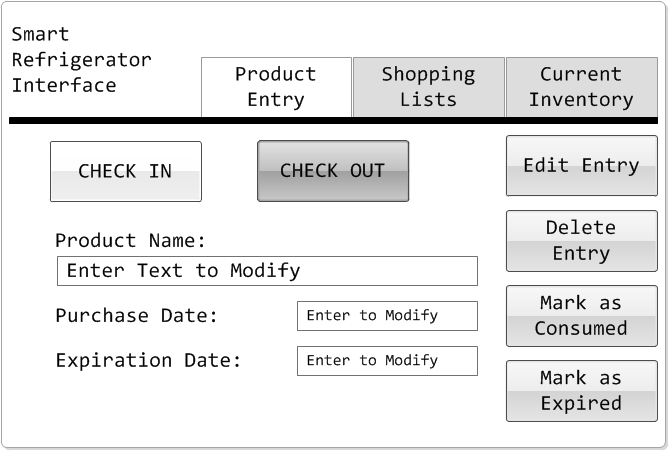
\includegraphics[scale=0.5]{MockUp1}
\label{mock1}
\end{center}
\end{figure}

\begin{figure}[h!]
\begin{center}
\caption{Shopping List Tab Layout}
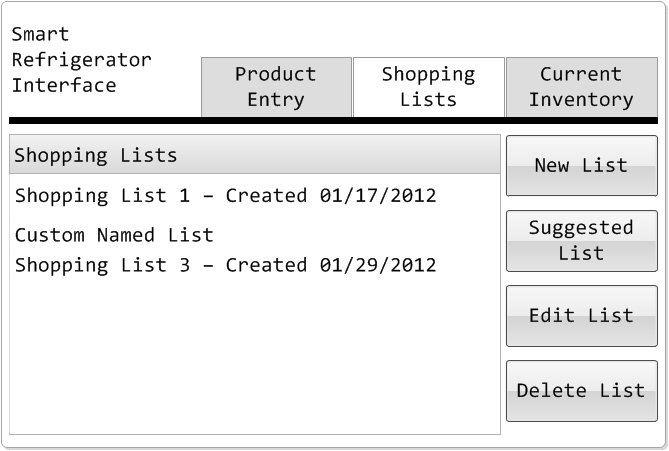
\includegraphics[scale=0.5]{MockUp2}
\label{mock2}
\end{center}
\end{figure}

\begin{figure}[h!]
\begin{center}
\caption{Current Inventory Tab Layout}
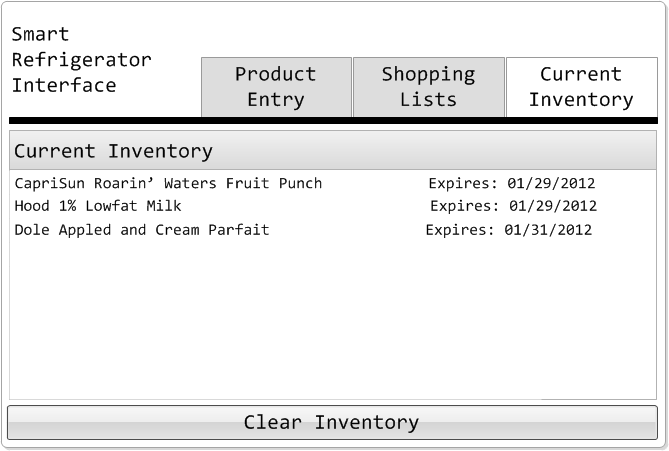
\includegraphics[scale=0.5]{MockUp3}
\label{mock3}
\end{center}
\end{figure}

\begin{figure}[h!]
\begin{center}
\caption{Expiration Warning Pop-Up Layout}
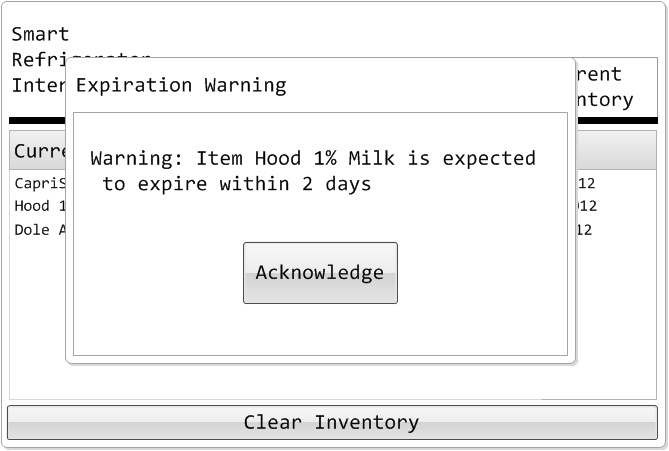
\includegraphics[scale=0.5]{MockUp4}
\label{mock4}
\end{center}
\end{figure}

\pagebreak
\section{Considerations}
The Smart Refrigerator system proposed is a step toward promoting sustainability and good stewardship of natural resources. Both the New York Times article mentioned in the statement of needs, and other reports \cite{times}\cite{aol}, indicate that approximately 27\% of all food available for consumption is lost to waste. A study published by the UN Food and Agriculture Organization declares the global percentage is even higher, a  total 1.3 billion tons or 33\% overall \cite{dutch}. The system designed will increase awareness about expiring items, with the goal of reducing these figures. Hugh Collins from AOL News speculates that food waste is dismissed subconsciously; many foods are cheap and the average consumer does not think about the cost of these small wastes aggregated \cite{aol}. By providing reminders to the user the Smart Refrigerator can remedy this source of waste by keeping the user aware of all their purchases. Expiration of foods products themselves is not the only source of waste involved with grocery shopping. Making unnecessarily frequent trips to store for forgotten or unexpected items also wastes resources. The shopping list recommendations provided by the Smart Refrigerator will hopefully mitigate waste here as well. A final consideration of the system is health and safety, by providing reminders about expiring products the risk of eating expired products will hopefully be decreased. 

\section{Cost Estimates}
We have submitted a proposal to the ARM student design contest requesting a BeagleBoard-xM and power adapter. If our proposal is accepted we will be able to obtain these parts at no cost. We also already own many of the principle system components, the dorm room refrigerator, android smart phone, and LCD display will all not need to be purchased.
\begin{table}[h!]
\begin{center}
\caption{Cost Table}
\label{tab:cost}
\begin{tabular}{| p{2.5in} | p{1.75in} |p{1.75in} |}
\hline
Part & Retail Cost & Our Cost \\
\hline
BeagleBoard-xM & \$149 & \$0 \\
\hline
BeagleBoard-xM Power Adapter & \$14.87 & \$0 \\
\hline
Dorm Room Refrigerator & \$100 & \$0 \\
\hline
Android Smart Phone & \$100 & \$0  \\
\hline
LCD Display & \$80  & \$0 \\
\hline
UPC Barcode Scanner & \$35 & \$35 \\
\hline
USB Keyboard/Keypad & \$10 & \$10 \\
\hline
\hline
\textbf{Total Cost} & \$488.87 & \$45 \\
\hline
\end{tabular}
\end{center}
\end{table}

\section{Testing Strategy}
Preliminary testing will focus on the BeagleBoard itself and its ability to interact with the desired peripherals.  The system will require an LCD screen, a USB barcode scanner, a network connection, and a keypad.  Basic functionality of these components will be tested thoroughly during development, as well as during final system testing. 
\newline \quad \newline
The SQL database used to store all data for the system will be tested once the core of the user application has been coded.  Test scripts will be written to populate the databases with fake data in order to ensure that the database is configured as desired, and to verify that the user application is properly communicating with the database alongside the web interface.
\newline \quad \newline
The main testing focus will be on the user application, both the software running on the base station as well as the web and Android interfaces.  Unit testing will be performed during development of each component, as well as integration testing of the final application.  Testing will focus on usability of the interface, accuracy of expiration date prediction and shopping list recommendations, and communication with the database. 
\newline \quad \newline
The web and mobile interfaces will have their own set of tests, focused on basic functionality and interoperability on various platforms.  The web interface will be tested on the most popular browsers (Google Chrome, Firefox, and Internet Explorer), as well as some of the most popular mobile platforms (Android, WebOS, and iOS).  The Android interface will need to be tested on various versions of the operating system.  At a minimum, major versions between 2.1 and 4.0 will be tested.  
\newline \quad \newline
As a final test, someone not involved in the project will test the system for usability as an end-user.

\section{Risks}
\subsection{Potential Difficulties}
\noindent There are a few things that could present difficulties as this project is implemented. The first is determining an accurate method to predict when a user is likely to purchase a food item. This requires statistical analysis of every food item which, in turn, requires a non-trivial amount of processing power. This brings us to the next challenge: finding an appropriate processing platform. It must be small, but have enough memory to store the product database, enough processing power to host the web service and calculate the product statistics, enough peripheral ports for the scanner and a small keypad, and have the ability to drive a display. The display is a third challenge, as it must be large enough to be useful, without increasing the power draw of the device or the overall cost. 

\subsection{Sources of Failure}
\noindent The three challenges listed above are also possible sources of failure. If the statistical analysis cannot be run on our platform, whether by processing power or other limitations, then there will be no way to know when to suggest that the user add an item to a grocery list. If the analysis is done improperly, the suggestions will not aid the user or improve shopping habits. If there is no feasible display to use with the system, then there would be no way for the user to receive any feedback when items were scanned in. If the bar code was misread, then the wrong item would be added to the database and the user would have no way of knowing. Finally, if there is not platform powerful enough or robust enough for the system, then the system would not be able to perform as required, and features and functionality would be severely limited.

\subsection {Contingency Plans}
\noindent It is possible to limit or even eliminate the risks of such failures. The implementation of a web interface will allow a user to access the database and see what items have been scanned in, and make sure that no items were misread. Via this interface, the user will also be able to set default expiration dates and other information about the products they have purchased. That way, in case the display or statistical analysis are unavailable, some related but basic functionality will still be available to the user. To ensure that the processing platform is robust enough, various requirements were set which defined the number of peripheral ports, the processor power, and display capabilities.

\subsection {Analysis}
\noindent In order to determine the best course of action in each case, analysis was done on each risk point. A number of display methods were investigated and compared, as well as a number of different processing platforms. Each comparison showcased the benefits and drawbacks of each item, and the best solution was decided upon in a way that was as empirical as possible. To determine the best method of statistical analysis, actual shopping data was collected and analyzed in a variety of different ways to find a model that matched, as closely as possible, the real world shopping habits of the user. With such methods implemented, the device will be able to accurately provide item suggestions.

\section{Milestones}
\begin{table}[h!]
\caption{Table of Milestones}
\begin{center}
\begin{tabular}{| p{6 cm} | p{4.5 cm} | p{4.5 cm}|}
%\begin{tabular}{|l|l|l|}
\hline
\textbf{Milestone} & \textbf{Scheduled Completion Date} & \textbf{Assigned} \\
\hline
Board Procurement & February 10, 2012 & Steven Strapp\\
\hline
Operating System running on board & February 17, 2012 & Ben Reeves \\
\hline
Peripherals properly interfacing with board & February 24, 2012 & Dustin Stroup \\
\hline
Basic UI, suitable for debugging & March 2, 2012 & Ben Reeves\\
\hline
Database I/O, proper reading from scanner & March 2, 2012 & Steven Strapp \\
\hline
Web interface operational & March 2, 2012 & Dustin Stroup \\
\hline
User profiling and Statistical Analysis & March 9, 2012 & Steven Strapp \\
\hline
Shopping lists, item modification, basic settings & March 9, 2012 & Ben Reeves \\
\hline 
Mobile application functional & March 16, 2012 & Dustin Stroup \\
\hline
Integration and System Testing & March 30, 2012 & Ben Reeves \\
\hline

\end{tabular}
\label {MilestoneTable}
\end{center}
\end{table}

\pagebreak

\addcontentsline{toc}{section}{10\hspace{.090in} References}
\begin{thebibliography}{9}
\bibitem{times}
Martin, Andrew. ``One Country's Table Scraps, Another Countr'ys Meal." New York Times. N.p., 18 May 2008. Web. 26 Jan 2012. 
\url{http://www.nytimes.com/2008/05/18/weekinreview/18martin.html?pagewanted=all}.
\bibitem{lg}
Ridden, Paul. ``LG launches first Smart-Grid appliance: the Smart Fridge." gizmag. N.p., 27 Apr 2011. Web. 29 Jan 2012. \url{<http://www.gizmag.com/lg-smart-fridge/18502/>}.
\bibitem{aol}
Collins, Hugh. ``Study: US Food Waste Is a Huge Energy Drain." AolNews. N.p., 02 Oct 2010. Web. 29 Jan 2012. \url{<http://www.aolnews.com/2010/10/02/study-american-food-waste-is-a-huge-energy-drain/>}.
\bibitem{dutch}
Ramaker, Rob. ``Food waste is hard to combat." Resource. N.p., 26 Jan 2012. Web. 29 Jan 2012. \url{<http://resource.wur.nl/en/wetenschap/detail/food_waste_is_hard_to_combat/>}.
 \end{thebibliography}

\end{document}